\documentclass[tikz,border=8pt]{standalone}
\usepackage{tikz}
\usepackage{xcolor}
\usetikzlibrary{positioning,arrows.meta}
\definecolor{ink}{HTML}{16140F}
\definecolor{cream}{HTML}{F6F4F1}
\definecolor{honey}{HTML}{F0B429}
\begin{document}
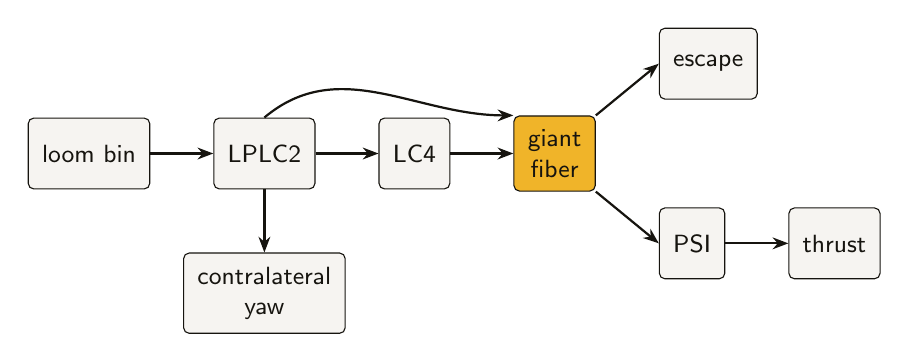
\begin{tikzpicture}[
  font=\sffamily,
  box/.style={draw=ink, fill=cream, text=ink, rounded corners=2pt, align=center, inner sep=5pt, font=\sffamily\small, minimum height=9mm},
  hot/.style={draw=ink, fill=honey, text=ink, rounded corners=2pt, align=center, inner sep=5pt, font=\sffamily\small, minimum height=9mm},
  arr/.style={-{Stealth[length=2mm]}, thick, draw=ink}
]
  \node[box] (bin) {loom bin};
  \node[box, right=8mm of bin] (lplc) {LPLC2};
  \node[box, right=8mm of lplc] (lc) {LC4};
  \node[hot, right=8mm of lc] (gf) {giant\\fiber};
  \node[box, above right=2mm and 8mm of gf] (esc) {escape};
  \node[box, below right=2mm and 8mm of gf] (psi) {PSI};
  \node[box, right=8mm of psi] (th) {thrust};
  \node[box, below=8mm of lplc] (yaw) {contralateral\\yaw};
  \draw[arr] (bin) -- (lplc);
  \draw[arr] (lplc) -- (lc);
  \draw[arr] (lc) -- (gf);
  \draw[arr] (lplc.north) to[out=40,in=180] (gf.north west);
  \draw[arr] (gf.north east) -- (esc.west);
  \draw[arr] (gf.south east) -- (psi.west);
  \draw[arr] (psi) -- (th);
  \draw[arr] (lplc.south) -- (yaw.north);
\end{tikzpicture}
\end{document}
